\documentclass[runningheads,a4paper]{llncs}

\usepackage[utf8]{inputenc}

\usepackage{amssymb}
\setcounter{tocdepth}{3}
\usepackage{graphicx}

\newcommand{\keywords}[1]{\par\addvspace\baselineskip
\noindent\keywordname\enspace\ignorespaces#1}

\usepackage{pifont} 
\usepackage[utf8]{inputenc}
\usepackage{enumitem}
\usepackage[hyphens]{url}
\usepackage[pdftex,urlcolor=black,colorlinks=true,linkcolor=black,citecolor=black]{hyperref}
\def\sectionautorefname{Section}
\def\subsectionautorefname{Subsection}

% listings and Verbatim environment
\usepackage{fancyvrb}
\usepackage{relsize}
\usepackage{listings}
\usepackage{verbatim}
\newcommand{\defaultlistingsize}{\fontsize{8pt}{9.5pt}}
\newcommand{\inlinelistingsize}{\fontsize{8pt}{11pt}}
\newcommand{\smalllistingsize}{\fontsize{7.5pt}{9.5pt}}
\newcommand{\listingsize}{\defaultlistingsize}
\RecustomVerbatimCommand{\Verb}{Verb}{fontsize=\inlinelistingsize}
\RecustomVerbatimEnvironment{Verbatim}{Verbatim}{fontsize=\defaultlistingsize}
\lstset{frame=lines,captionpos=b,numberbychapter=false,escapechar=§,
        aboveskip=2em,belowskip=1em,abovecaptionskip=0.5em,belowcaptionskip=0.5em,
        framexbottommargin=-1em,basicstyle=\ttfamily\listingsize\selectfont}

% use Courier from this point onward
\let\oldttdefault\ttdefault
\renewcommand{\ttdefault}{pcr}
\let\oldurl\url
\renewcommand{\url}[1]{\inlinelistingsize\oldurl{#1}}

\usepackage[usenames,dvipsnames,svgnames,table]{xcolor}
\lstdefinelanguage{JavaScript}{
  keywords={push, typeof, new, true, false, catch, function, return, null,
    catch, switch, var, if, in, while, do, else, case, break, div, script, video},
  keywordstyle=\bfseries,
  ndkeywords={class, export, boolean, throw, implements, import, this},
  ndkeywordstyle=\color{darkgray}\bfseries,
  identifierstyle=\color{black},
  sensitive=false,
  comment=[l]{//},
  morecomment=[s]{/*}{*/},
  morecomment=[s]{<!--}{-->},  
  commentstyle=\color{darkgray},
  stringstyle=\color{gray},
  morestring=[b]',
  morestring=[b]"
}
\lstset{breaklines=true}

% linewrap symbol
\usepackage{color}
\definecolor{grey}{RGB}{130,130,130}
\newcommand{\linewrap}{\raisebox{-.6ex}{\textcolor{grey}{$\hookleftarrow$}}}

% todo macro
\usepackage{color}
\newcommand{\todo}[1]{\noindent\textcolor{red}{{\bf \{TODO}: #1{\bf \}}}}

\def\JSONLD{\mbox{JSON-LD}}

\hyphenation{WebVTT}

\def\JSONLD{\mbox{JSON-LD}}

\begin{document}

\mainmatter  % start of an individual contribution

% first the title is needed
\title{Projet ``Spectacle en ligne(s)''---Livrable L4.1.2\\``Modèles documentaires pour les hypervidéos sur le web''}

% a short form should be given in case it is too long for the running head
\titlerunning{``Spectacle en ligne(s)''---Livrable L4.1.2}

% the name(s) of the author(s) follow(s) next
\author{
  Thomas Steiner\textsuperscript{1} \and
  Pierre-Antoine Champin\textsuperscript{1} \and \\
  Benoît Encelle\textsuperscript{1}\and
  Yannick Prié\textsuperscript{2}
}
%
\authorrunning{Steiner, Champin, Encelle, and Prié}
% (feature abused for this document to repeat the title also on left hand pages)

% the affiliations are given next
\institute{
  \textsuperscript{1}CNRS, Université de Lyon, LIRIS -- UMR5205, Université Lyon~1, France\\
  \email{\{tsteiner, pierre-antoine.champin\}@liris.cnrs.fr, benoit.encelle@univ-lyon1.fr}\\
  \textsuperscript{2}CNRS, Université de Nantes, LINA -- UMR 6241, France\\
  \email{yannick.prie@univ-nantes.fr}
}

\maketitle

\begin{abstract}
\keywords{Annotation, description model, hypervideo}
\end{abstract}

\section{Introduction}

The term \emph{hypervideo} is commonly used to refer to
\textit{``a~displayed video stream that contains embedded user-clickable anchors''}%
~\cite{sawhney1996hypercafe,smith2002extensible}.
In a~2006 article in \emph{The Economist}, the authors write 
\textit{``[h]yperlinking video involves the use of ``object-tracking'' software
to make filmed objects, such as cars, clickable as they move around.
Viewers can then click on items of interest in a~video
to watch a related clip; after it has played,
the original video resumes where it left off.
To inform viewers that a~video is hyperlinked,
editors can add highlights to moving images, use beeps as audible cues,
or display still images from hyperlinked videos
next to the clip that is currently playing''}~\cite{economist2006hypervideo}.
In standard literature, hypervideo is considered a~logical consequence
of the related concept of \emph{hypertext}.

In this deliverable, we will look at
description models for hypervideos on the Web.
This topic is also a~core area of research of the currently active
European research project ``LinkedTV''~\cite{linkedtv2012hypervideo}.
Further, a~bachelor's thesis by Jäger specifically focuses on interface aspects
of hypervideos on the Web~\cite{jaeger2012hypervideo}.

Our main objective is to facilitate the publication and consumption
of Linked Data for videos from the \emph{``Spectacle en ligne(s)''} corpus.
Therefore, in the first part of this deliverable,
we will propose an annotation model
based on invisible metadata timed text track cues for videos.
This annotation model is based on a~number of enabling technologies,
which we will outline in the following.
In the second part, we will present an online Read/Write-enabled editor
that implements this annotation model.
In the third part of the deliverable,
we will introduce a~description model for hypervideos
based on Web Components.

\section{Video Annotation Model}

\subsection{Technologies Overview}

For our approach to online video annotation,
we make use of a~young---yet mature
when looked at from an implementation viewpoint---%
stack of enabling technologies that we will introduce in the following.

\subsubsection{Web Video Text Tracks format (WebVTT)}

The Web Video Text Tracks format (WebVTT,~\cite{pfeiffer2013webvtt})
is intended for marking up external text track resources mainly
for the purpose of captioning video content.
The recommended file extension is \texttt{vtt},
the MIME type is \texttt{text/vtt}.
WebVTT files are encoded in UTF-8 and
start with the required string \texttt{WEBVTT}.
Each file consists of items called \emph{cues}
that are separated by an empty line.
Each cue has a~start time and an end time in
\texttt{hh:mm:ss.milliseconds} format,
separated by a~stylized ASCII arrow \texttt{-}\texttt{->}.
The cue payload follows in the line after the cue timings part
and can span multiple lines.
Typically, the cue payload contains plain text,
but can also contain textual data serialization formats like JSON,
which later on in the paper we will show is essential
for our proposed approach to semantic video annotation.
Spans of text associated with a~specific voice can be annotated
in form of WebVTT cue voice spans.
A~WebVTT voice tag, denoted by \texttt{<v VOICE>}, has a~value,
which is the name of the voice.
Cues optionally can have unique WebVTT identifiers.

\begin{table}[b!]\footnotesize
\begin{tabular}{ r p{9.5cm} }
\textbf{WebVTT Kind} & \textbf{Description and Default Behavior}\\

\texttt{subtitles} & Transcription or translation of speech,
suitable for when sound is available but not understood.
Overlaid on the video.\\

\texttt{captions} & Transcription or translation of the dialogue,
sound effects, and other relevant audio information,
suitable for when sound is unavailable or not clearly audible.
Overlaid on the video;
labeled as appropriate for the hard-of-hearing.\\

\texttt{descriptions} & Textual descriptions of the video component
of the media resource, intended for audio synthesis
when the visual component is obscured, unavailable, or unusable.
Synthesized as audio.\\

\texttt{chapters} & Chapter titles, intended to be used for navigating
the media resource. Displayed as an interactive (potentially nested)
list in the user agent's interface.\\

\texttt{metadata} & Metadata intended for use from script context.
Not displayed by user agent.\\
\end{tabular}
  \caption{WebVTT text track kinds in HTML5~\cite{berjon2013html5}}
  \label{table:texttrackkinds}
\end{table}

WebVTT-compliant Web browsers~\cite{dutton2012trackelement}
support five different kinds of
WebVTT tracks: \emph{subtitles}, \emph{captions},
\emph{descriptions}, \emph{chapters}, and \emph{metadata},
all specified in HTML5~\cite{berjon2013html5}.
In this paper, we especially focus on
text tracks of kind \texttt{metadata}
that are meant to be used from a~scripting context and
that are not displayed by the user agent.

Both the HTML5 \texttt{<audio>} and \texttt{<video>} elements
have a~\texttt{textTracks} property
that returns a~\texttt{TextTrackList} of
\texttt{TextTrack} members, each of which correspond
to individual <track> elements.
A~\texttt{TextTrack} has a~\texttt{cues} property
that returns a~\texttt{TextTrackCueList} of individual
\texttt{TextTrackCue} items.
Cue data is accessible via properties like
\texttt{startTime}, \texttt{endTime} and,
most importantly, \texttt{text} to obtain a~cue's payload.
When the payload is in JSON format,
it can be parsed via the
\texttt{JSON.parse()} function.

When a~media resource like a~video or audio is playing,
JavaScript events of the \texttt{TextTrack} and \texttt{TextTrackCue}
elements fire automatically when the \texttt{currentTime}
of the media resource matches
a~cue's \texttt{startTime} or \texttt{endTime}.
\texttt{TextTrack} elements fire \texttt{oncuechange} events,
whereas \texttt{TextTrackCue} elements fire
\texttt{onenter} and \texttt{onexit} events.
JavaScript applications can subscribe to these events.
Important for us, both \texttt{TextTrack} and
\texttt{TextTrackCue} elements
can be dynamically generated via JavaScript.

\subsubsection{\JSONLD}

The \emph{JavaScript Object Notation}%
\footnote{JavaScript Object Notation: \url{http://json.org/}}
(JSON)
is a~(despite the name) language-independent textual syntax
for serializing objects, arrays, numbers, strings, booleans, and null.
\emph{Linked Data}~\cite{bizer2009linkeddata}
describes a~method of publishing structured data
so that it can be interlinked and become more useful,
which builds upon standard Web technologies such as HTTP, RDF and URIs.
Based on top of JSON, the
\emph{JavaScript Object Notation for Linked Data}
(\JSONLD,~\cite{sporny2013jsonld}) is a~method for transporting
Linked Data with a~smooth upgrade path from JSON to \JSONLD.
\JSONLD~properties like \texttt{title} can be mapped to taxonomic
concepts (like \texttt{dc:title}) via so-called data contexts.
We use \JSONLD\ for semantically rich content
in the payload of \texttt{TextTrackCue}s, shown in
\autoref{listing:webvtt}.
The referenced local context defines the semantics.

\subsubsection{Media Fragments URI}

Media Fragments URI~\cite{troncy2012mediafragments}
specifies a~syntax for constructing media fragments URIs
and explains how to handle them over the HTTP protocol.
The syntax is based on the specification of
name-value pairs that can be used in URI query strings
and URI fragment identifiers to restrict a~media resource
to a~certain fragment.
Media Fragments URI supports temporal and spatial media fragments.
The \emph{temporal dimension} is denoted
by the parameter name \texttt{t} and specified
as a~half-open interval with begin time and end time
that may also be omitted,
with the begin time defaulting to 0 seconds
and the end time defaulting to the media item's duration.
The \emph{spatial dimension} selects
a~rectangular area of pixels from media items.
Rectangles can be specified as pixel coordinates or percentages.
Rectangle selection is denoted by the parameter name \texttt{xywh}.
The value is either \texttt{pixel:} or \texttt{percent:}
(defaulting to \texttt{pixel:})
followed by four comma-separated integers.
The integers denote $x$, $y$, $width$, and $height$ respectively,
with $x = 0$ and $y = 0$ being the top left corner of the media item.
If \texttt{percent:} is used, $x$ and $width$ are interpreted
as percentage of the width of the original media item,
$y$ and $height$
of the original height.

\subsubsection{Ontology for Media Resources}

The Ontology for Media Resources~\cite{lee2012mediaontology}
serves to bridge different description methods of media resources
and to provide a~core set of descriptive properties.
It also defines mappings to common metadata formats.
Combined with Media Fragments URI,
this allows for making ontologically anchored statements
about media items and fragments thereof.

\begin{lstlisting}[caption={Sample WebVTT metadata file},
  label=listing:webvtt, float=t!]
WEBVTT

cue1
00:00:00.000 --> 00:00:12.000
{
  "@context": "http://ex.org/local_context",
  "tags": ["wind scene", "opening credits"],
  "contributors": ["http://ex.org/sintel"]
}
\end{lstlisting}

\begin{lstlisting}[caption={Generated \JSONLD~for the Web of Data, see
    \url{http://bit.ly/webvtt-jsonld} for the RDF triples},
  label=listing:jsonld, float=t!]
{
  "@context": "http://ex.org/global_context",
  "@id": "http://ex.org/video",
  "@type": "MediaResource",
  "hasFragment": [{
    "@id": "http://ex.org/video#t=0,12",
    "@type": "MediaFragment",
    "@context": "http://ex.org/local_context",
    "tags": ["wind scene", "opening credits"],
    "contributors": ["http://ex.org/sintel"]
  }]
}
\end{lstlisting}

\subsection{General Concepts of the Annotation Model}

Our annotation model uses subject-predicate-object expressions.
An annotation is thus a~single triple.
The possible values for the \emph{subject} can be \emph{(i)}~the video
URI itself or---in case of multiple URIs for a~video available
in different encodings with multiple \texttt{<source>} tags---%
the URI with fragment identifier of the \texttt{<video>} tag
that then requires a~unique \texttt{id} attribute,
\emph{(ii)}~the Media Fragment URI of a~temporal and/or spatial
media fragment of the original media item.
We have no constraints in place for the \emph{predicate},
which determines the annotation type, and the \emph{object}.
In our interpretation layer responsible for the video view,
we thus make an open world assumption
by supporting a~set of pre-defined values for predicate and object
listed below, and ignoring unknown ones.
This permits others to extend---or even completely replace---%
our interpretation layer.
If a~\texttt{TextTrackCue} has a~WebVTT identifier,
we use it to address its annotations
via the metadata track's URI
and corresponding cue fragment identifier,
allowing for meta annotations of annotations, \emph{e.g.},
to attach provenance or license information to them.

\subsection{Related Work}

The online video hosting platform YouTube%
\footnote{YouTube: \url{http://www.youtube.com/}}
lets video publishers add video annotations
in a~closed proprietary format%
~\cite{youtube2008annotations,youtube2010annotations}.
YouTube supports the following
annotation types: \emph{speech bubbles},
\emph{spotlights} for highlighting areas in a~video
that react on mouse-over,
\emph{notes} for creating pop-up boxes containing text,
\emph{titles} for creating text overlays to title a~video,
and \emph{labels} to call out
and name a~specific part of a~video.
Some types can contain \emph{links}
to other videos, the same video, channels, playlists,
or search results, as well as to actions
such as subscribe, compose message, and upload video response.
From 2009 to 2010, YouTube had a~feature called
Collaborative Annotations%
~\cite{fink2009collaborativeannotations}
that allowed video consumers to collaboratively
create video annotations.
Unlike the format of YouTube, our format is open and standards-based.
It was discontinued \textit{``to make room for even more new features''}%
~\cite{youtube2010annotations}.

In~\cite{vandeursen2012mediafragmentannotations},
Van Deursen \emph{et~al.}\ present a~system
that combines Media Fragments URI~\cite{troncy2012mediafragments}
and the Ontology for Media Resources~\cite{lee2012mediaontology}
in an HTML5~\cite{berjon2013html5}
Web application to convert rich media fragment annotations
into a~WebVTT~\cite{pfeiffer2013webvtt} file
that can be used by HTML5-enabled players
to show the annotations in a~synchronized way.
Their systems allows for linking, displaying, and
browsing of media fragments and
for providing structured annotations for media fragments.
Building on the work of Van Deursen \emph{et~al.},
we additionally allow for writing annotations by
letting annotators create WebVTT cues with an editor.

The Synchronized Multimedia Integration Language
(SMIL,~\cite{bulterman2006smil})
defines an XML-based language that allows authors
to write interactive multimedia presentations.
Using SMIL, an author can describe the temporal behavior
of a~multimedia presentation, associate hyperlinks
with media objects, and describe the layout
of the presentation on a~screen.
SMIL components can be used for integrating timing
into XHTML~\cite{pemberton2002xhtml}
and into SVG~\cite{ferraiolo2003svg}.
SMIL features are not commonly supported
in modern Web browsers and special plugins or native software
are required for their consumption,
albeit in 2002 there was a~mostly Microsoft-led attempt
in form of the HTML+TIME submission~\cite{schmitz1998htmltime}
\footnote{HTML+TIME for extending SMIL into Web browsers: \url{http://www.w3.org/TR/NOTE-HTMLplusTIME}}
and, based thereon, the XHTML+SMIL Profile%
\footnote{XHTML+SMIL Profile Note:
\url{http://www.w3.org/TR/XHTMLplusSMIL/}} note
~\cite{newman2002xhtmlsmil}
to integrate SMIL semantics with (X)HTML and CSS.
despite its initially active role in the W3C SMIL working group,
Microsoft later decided to cease SMIL support
due to a~perceived overlap with several existing standards.
Our approach is based on native browser technologies.

The Component-based Hypervideo Model
(CHM,~\cite{sadallah2012hypervideo})
proposes a~formal model for hypervideo documents
and offers a~practical framework that allows for
the design of Web-oriented hypervideos.
CHM annotations are defined as any kind of data associated to
a~logical spatiotemporal video fragment.
A~version of the proposed framework
has been released in form of the WebCHM prototype
that integrates with existing Web technologies
via a~declarative syntax.
Support for temporal semantics is ensured through
an implementation of SMIL Timesheets.%~\cite{vuorimaa2012timesheets}
\footnote{SMIL Timesheets:
\url{http://www.w3.org/TR/timesheets/}}
At comparable functionality, our approach is less complex
and entirely Web-based.

Popcorn.js\footnote{Popcorn.js: \url{http://popcornjs.org/}}
is an HTML5 JavaScript media framework
aimed at filmmakers, Web developers,
and users interested in creating
for the creation of media mixes
by adding interactivity and context to online video
by letting users link social media, feeds,
visualizations, and other content directly to moving images.
PopcornMaker%
\footnote{PopcornMaker: \url{https://popcorn.webmaker.org/}}
is an interactive Web authoring environment
that allows for videos to be annotated on a~video timeline.
While Popcorn media annotations are JavaScript-based,
our approach is based on indexable WebVTT files.

The Flash tool VideoANT~\cite{hosack2010videoant} by Hosack
was designed to create text-based annotations
integrated within the timeline of videos hosted online.
Annotations consist of subject and content and
are positioned based solely on start time.
Annotations can be exported as RSS, JSON, XML, and text.

\subsection{Discussion}

With our annotation approach, we leverage WebVTT
metadata tracks as a~means for tying semantically rich JSON-LD annotations
to temporal and/or spatial video fragments.
As each \texttt{<track>} element by pure definition is bound to
exactly one \texttt{<video>} element and as modern search engines
parse JSON-LD annotations,
a~unique relation of annotations to video content is made.
We show below that this is not the case for the two
popular online video annotation tools.

\subsubsection{Main Difference to Popcorn.js and PopcornMaker}

The Popcorn.js and PopcornMaker technology stacks
represent the state-of-the-art in online video annotation,
backed by the Mozilla Foundation
and organized in active open-source projects.%
\footnote{Popcorn.js on GitHub: \url{https://github.com/mozilla/popcorn-js}}%
\textsuperscript{,}%
\footnote{PopcornMaker on GitHub: \url{https://github.com/mozilla/popcorn.webmaker.org}}
We are by no means positioning our approach as superior,
yet we claim that Popcorn annotations have shortcomings
when it comes to indexability and semantic expressivity. 
We back this claim with an example
that can be seen in \autoref{listing:popcorn}.
In this example, two annotations, a~freeform footnote 
and an ambiguity-free reference to a~Wikipedia article, are added.
There is, however, no way to actually express the semantic concept
that the video fragment ranging from seconds 2 to 6 (or a~spatial fragment thereof) 
\texttt{foaf:depicts}%
\footnote{FOAF: \url{http://xmlns.com/foaf/spec/}} the person and actor
\texttt{dbp:George\_Clooney}.
In addition to that, the annotations are pure JavaScript source code
with---at least for search engines---no semantic connection
to the video in question.

\subsubsection{Main Difference to VideoANT}

VideoANT is a~Flash-based tool that requires a~browser plugin to run.
Search engines have rather limited support
for accessing data encoded in Flash.
\autoref{listing:videoant} shows the purely textual annotations
of subject and content analog to \autoref{listing:popcorn}
exported to the accessible JSON format.
Albeit VideoANT supports the export of annotations
in RSS, JSON, XML, and plain text,
this operation requires manually pressing a~button in the tool.
For search engines, there is no semantic connection
to the video in question.

\subsubsection{Our Approach}

Finally, \autoref{listing:webvttclooney} shows JSON-LD annotations
analog to \autoref{listing:popcorn} embedded in a~metadata track cue.
The Web browser intrinsically knows to which exact timespan
of which video this very cue is tied and search engines can interpret
the JSON-LD and, based on the \texttt{@context},
infer that \texttt{depicts} actually means \texttt{foaf:depicts}.

\begin{lstlisting}[caption={Popcorn.js example},
  label=listing:popcorn, float=t!, language=JavaScript]
<video id="video" src="http://ex.org/video.mp4">
</video>
<div id="footnote-container"></div>
<div id="wikipedia-container"></div>
<script>
  var pop = Popcorn("#video");
  pop.footnote({
      start: 2,
      end: 6,
      text: "In this scene: George Clooney",
      target: "footnote-container"
    });
  pop.wikipedia({
      start: 2,
      end: 6,
      src: "http://en.wikipedia.org/wiki/George§\linewrap§
          _Clooney",
      title: "George Clooney",
      target: "wikipedia-container"
    });    
</script>
\end{lstlisting}

\begin{lstlisting}[caption={VideoANT annotations analog to \autoref{listing:popcorn}},
  label=listing:videoant, language=JavaScript, float=t!]
{
  "ant": {
    "title": "Example Video",
    "url": "http://ex.org/video.mp4",
    "author": "Jon Doe (jon@doe.com)",
    "annotations": [{
      "annotation": {
        "subject": "In this scene",
        "content": "George Clooney",
        "author": "Jon Doe (jon@doe.com)",
        "seconds": 2
      }
    }, {
      "annotation": {
        "subject": "DBpedia link",
        "content": "http://dbpedia.org/resource/§\linewrap§
            George_Clooney",
        "author": "Jon Doe (jon@doe.com)",
        "seconds": 2
      }
    }]
  }
}
\end{lstlisting}

\begin{lstlisting}[caption={WebVTT annotations analog to \autoref{listing:popcorn}},
  label=listing:webvttclooney, float=t!]
WEBVTT

cue1
00:00:02.000 --> 00:00:06.000
{
  "@context": "http://ex.org/local_context",
  "depicts": ["http://dbpedia.org/resource/§\linewrap§
      George_Clooney"],
  "htmlOverlay": "<span>In this scene:</span>§\linewrap§
      <em>George Clooney</em>"
}
\end{lstlisting}

\section{Online Video Annotation Format and Editor}
\label{sec:online-video-annotation-format-and-editor}

We have implemented this annotation model
in form of an online demonstrator prototype.
The demonstrator interprets the existing metadata track for a~video
and reacts on annotations when the \texttt{currentTime}
of the media resource matches the
\texttt{startTime} or \texttt{endTime} of a~cue.
We call existing annotations \emph{Read} annotations.
Users can add \emph{Write} annotations
by creating new \texttt{TextTrackCue}s
at the desired start and end times
and by providing their \JSONLD~payloads.
The editor facilitates this task through a~graphical user interface, abstracting the underlying details.
\autoref{fig:webvtt-editor} shows a~screenshot of the WebVTT editor.
Newly generated annotations get directly interpreted
and can be persistently stored locally
or in the future remotely for collaborative editing.
We have developed a~WebVTT to \JSONLD~%
converter, capable of transforming WebVTT metadata tracks
following our annotation model
into \JSONLD~for the Web of Data.
This allows for straight-forward local annotation creation
with Semantic Web compliance upon global publication.

\subsubsection{Semantic Annotation Types}

Our \JSONLD\ context eases common annotation tasks
by defining the semantics of a~few useful JSON properties described below.
According to this context, \autoref{listing:webvtt} is interpreted as in
\autoref{listing:jsonld} (in \JSONLD) and \autoref{listing:rdftriples} (in RDF).
More advanced annotation tasks can be supported by extending the data context.

\begin{description}[leftmargin=*]
  \item[Plain Text Tags] Annotations of type
  \texttt{tags} allow for add\-ing plain text tags
  to a~media fragment.
  They are interpreted as Common Tag%
  ~\cite{commontag2009spec} format \texttt{ctag:label}.

  \item[Semantic Tags] Annotations of type
  \texttt{semanticTags} allow for adding semantic tags
  to a~media fragment.
  Unlike plain text tags, semantic tags are references to
  well-defined concepts complete with their own URIs.
  They are interpreted as Common Tag%
  ~\cite{commontag2009spec} format \texttt{ctag:means}.
  Spatiotemporal semantic tags allow for
  interesting Linked Data experiences
  if the tags point to well-connected concepts.

  \item[Contributors] The \texttt{contributors} annotation type
  allows for denoting the contributors in a~media fragment, like its actors.
  They are interpreted as
  Ontology for Media Resources~\cite{lee2012mediaontology}
  format \texttt{ma:hasContributor}.

  \item[Summary] The \texttt{summary} annotation type
  allows for summarizing a~media fragment
  (note, not the whole video like kind \emph{description} tracks)
  with plain text.
  They are interpreted as  
  \texttt{ma:description}~\cite{lee2012mediaontology}.
\end{description}

\subsubsection{Presentation-Oriented Annotation Types}

Presentation-oriented annotations,
similar to temporal style sheets,
do not generate RDF data,
but only impact the way videos get presented.\\

\begin{description}[leftmargin=*]
  \item[Visual Effect] Annotations of
  type \texttt{visualEffect} allow for applying visual effects
  in the syntax of Cascading Style Sheets%
  \footnote{Cascading Style Sheets:
  \url{http://www.w3.org/Style/CSS/}} (CSS)
  to a~media fragment, \emph{e.g.},
  filters, zoom, transparency,
  and 2D/3D transformations and animations.

  \item[Audial Effect] The \texttt{audialEffect} annotation type
  allows for applying audial effects to a~media fragment.
  Currently, we support modifying the volume
  from~0 to~1.

  \item[Playback Rate] The \texttt{playbackRate}
  annotation type allows for specifying the effective
  playback rate of a~media fragment.
  The playback rate is expressed as a~floating point
  multiple or fraction of the intrinsic video speed.

  \item[HTML Overlay] Via the \texttt{htmlOverlay}
  annotation type, overlays in
  freeform HTML code can be added to a~media fragment.
  Examples are graphical, textual, or combined overlays
  that can contain links to (temporal fragments of)
  other videos or within the current video.
\end{description}

\begin{lstlisting}[caption={Generated \JSONLD\ file based on the WebVTT file 
    shown in \autoref{listing:webvtt}~(flat interpretation)},
  label=listing:jsonld, float=t!]
{
  "@context": "http://champin.net/2014/linkedvtt/context.json",
  "@id": "http://ex.org/metadata.vtt", 
  "@type": "VideoMetadataDataset",
  "video": "http://ex.org/video", 
  "cues": [{
    "@id": "#id=cue1",
    "fragment": {
      "@context": "http://champin.net/2014/linkedvtt/demonstrator-context.json", 
      "@id": "http://ex.org/video#t=0:0.0,0:12.0", 
      "tags": ["wind scene", "opening credits"],
      "contributors": ["http://ex.org/sintel"]
    }
  }]
}
\end{lstlisting}

\begin{lstlisting}[caption={RDF triples based on the \JSONLD\ code from \autoref{listing:jsonld}},
  label=listing:rdftriples, float=t!]
<http://ex.org/metadata.vtt> <http://www.w3.org/1999/02/22-rdf-syntax-ns#type> <http://ex.org/VideoMetadataDataset> .
<http://ex.org/metadata.vtt> <http://champin.net/2014/linkedvtt/onto#hasCue> <http://ex.org/metadata.vtt#id=cue1> .
<http://ex.org/metadata.vtt#id=cue1> <http://champin.net/2014/linkedvtt/onto#describesFragment> <http://ex.org/video#t=0:0.0,0:12.0> .
<http://ex.org/video#t=0:0.0,0:12.0> <http://commontag.org/ns#label> "wind scene" .
<http://ex.org/video#t=0:0.0,0:12.0> <http://commontag.org/ns#label> "opening credits" .
<http://ex.org/video#t=0:0.0,0:12.0> <http://www.w3.org/ns/ma-ont#hasContributor> <http://ex.org/sintel> .
\end{lstlisting}
  
\subsection{Interpretation Layer}

In our WebVTT editor,
we propose an interpretation layer
capable of dealing with the herein defined annotation types. 
We thus make an open world assumption
by supporting a~set of pre-defined values for predicate and object
listed below, and ignoring unknown ones.
This permits others to extend---or even completely replace---%
our interpretation layer.
If a~\texttt{TextTrackCue} has a~WebVTT identifier,
we use it to address its annotations
via the metadata track's URI
and corresponding cue fragment identifier,
allowing for meta annotations of annotations, \emph{e.g.},
to attach provenance or license information to them.

\begin{figure*}[hbt]
  \centering
  \fbox{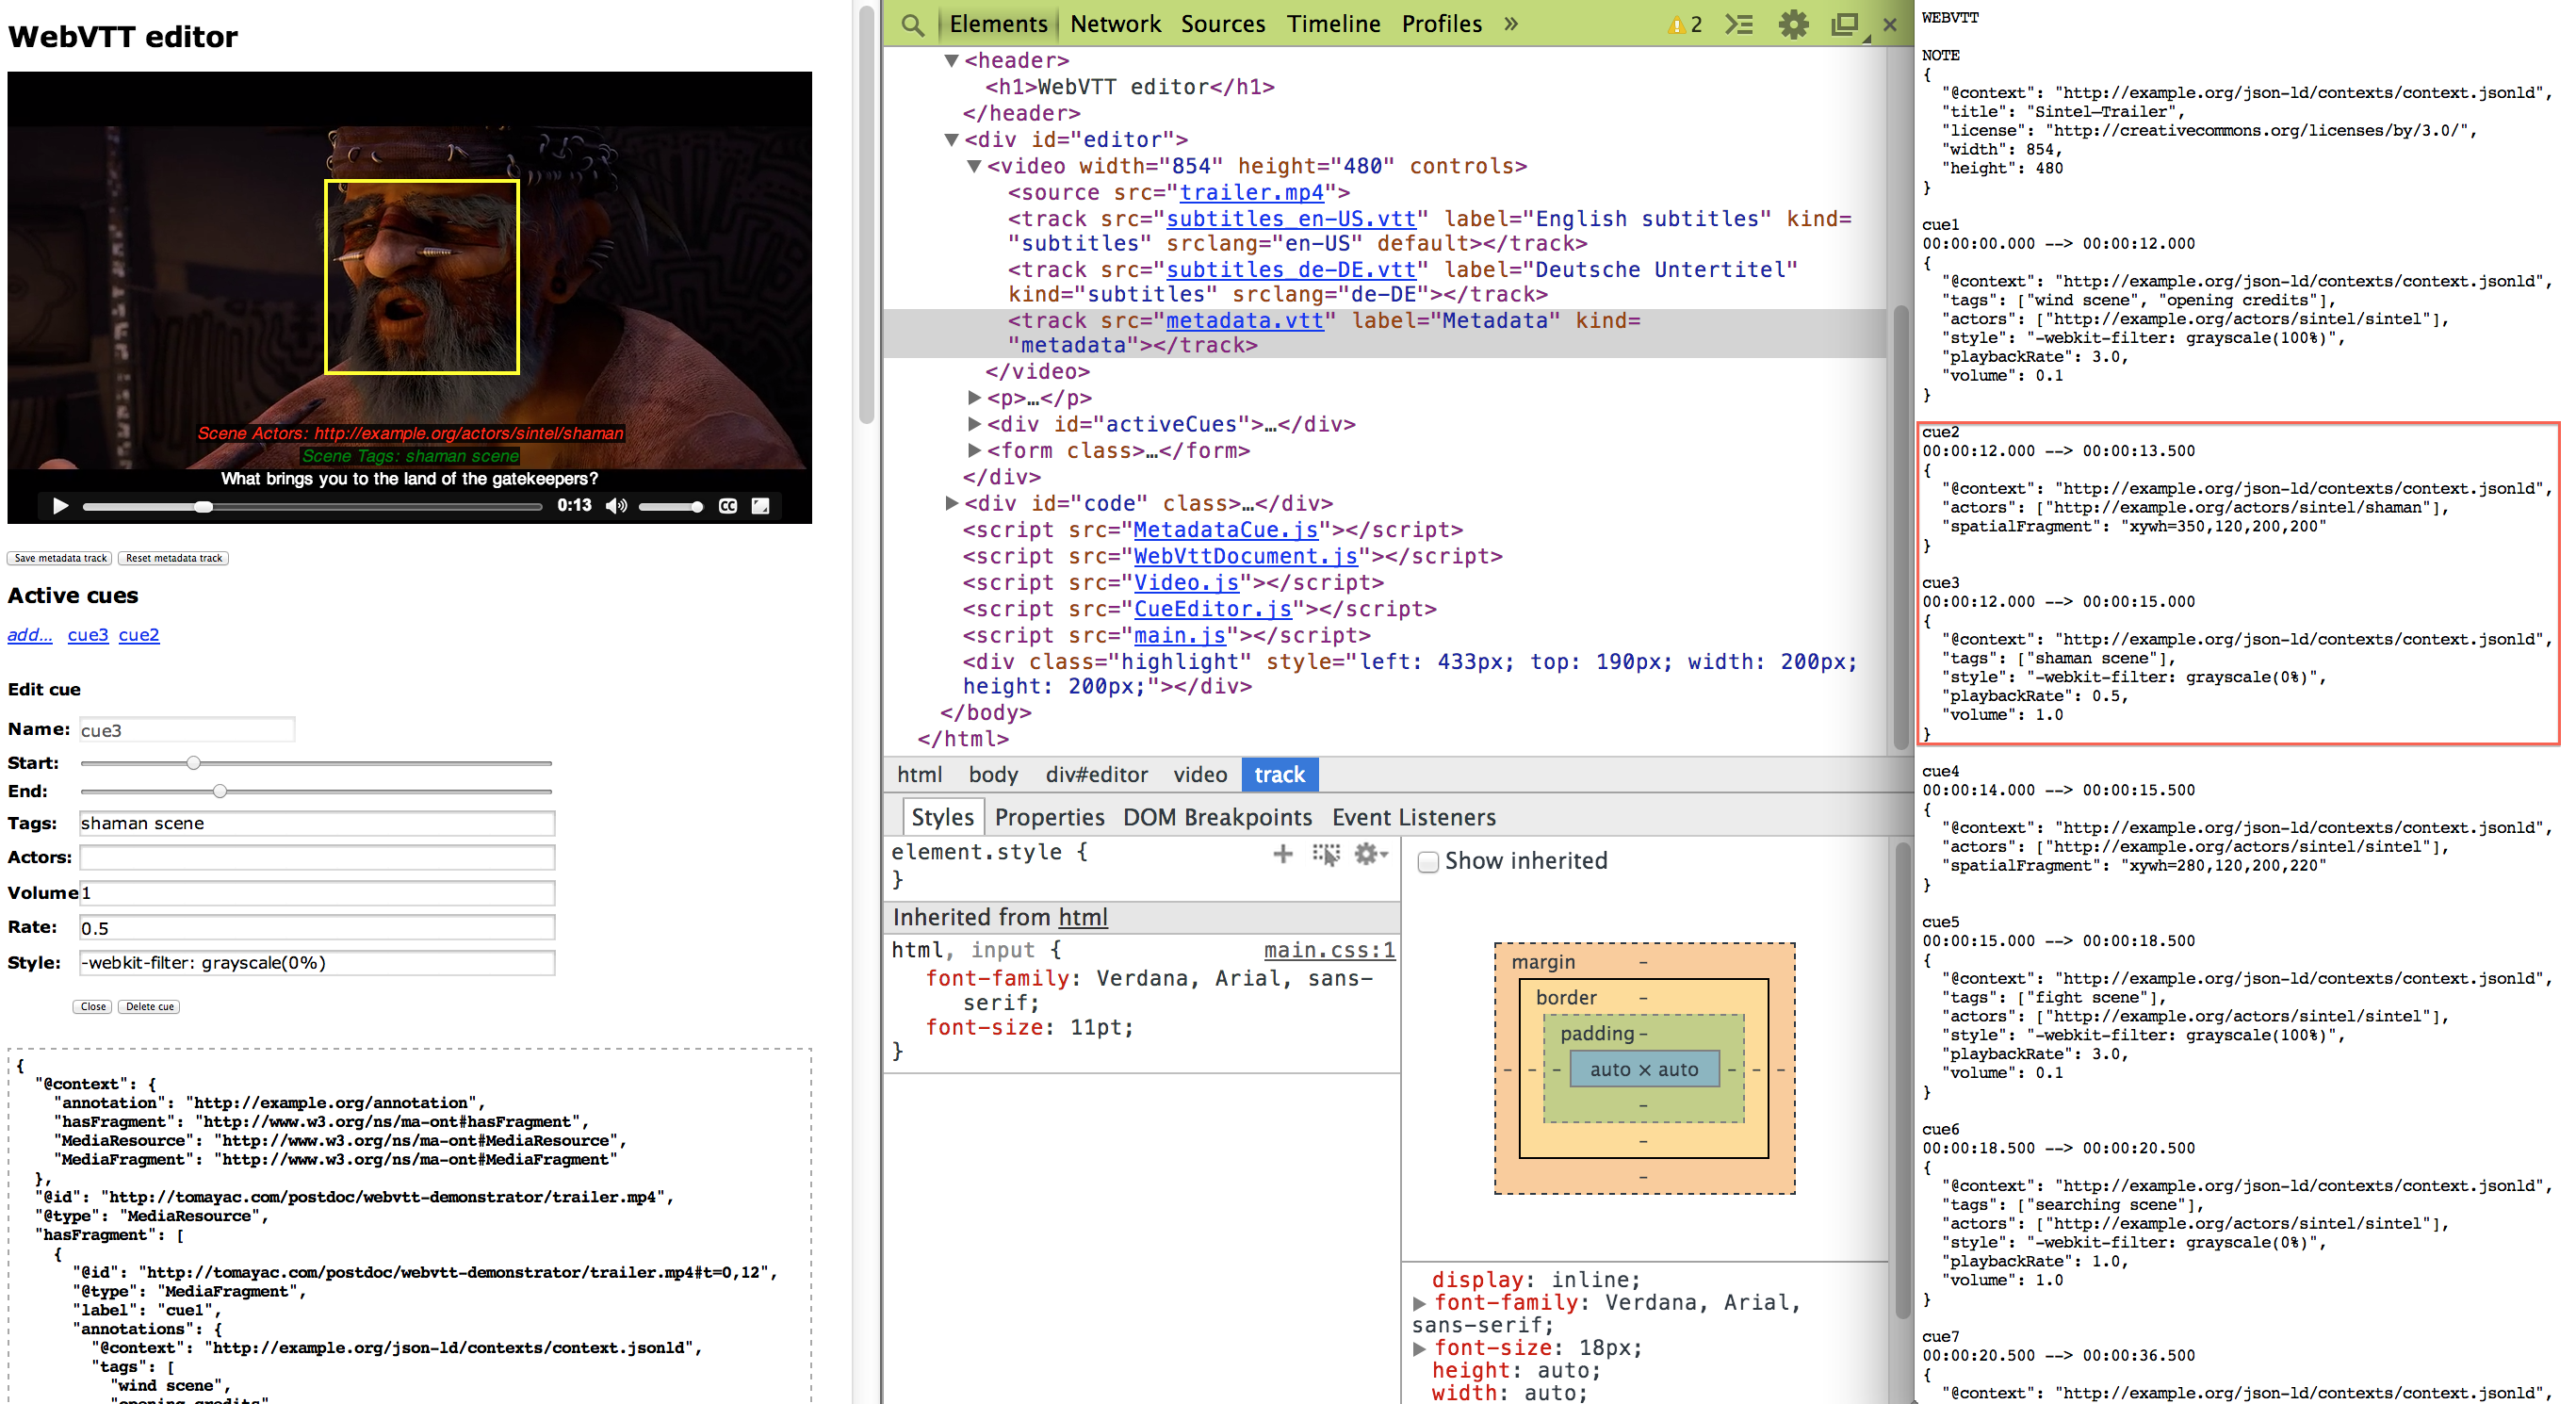
\includegraphics[width=\linewidth]{weaving-the-web(vtt)-of-data}}
  \caption{WebVTT editor interpreting the~spatiotemporal annotation ``cue2''
    that identifies the highlighted spatial fragment as \texttt{ex:actors/sintel/shaman};
    while in parallel modifying ``cue3'' with tag, volume, playback rate,
    and style (\ding{172} left: Graphical User Interface with \JSONLD\ debug view,
  \ding{173} center: Chrome Developer Tools with highlighted
  \texttt{<track src="metadata.vtt" kind="metadata">} tag,
  \ding{174} right: raw WebVTT file \texttt{metadata.vtt} with highlighted ``cue2'' and ``cue3'')}
  \label{fig:webvtt-editor}
\end{figure*}

\section{Hypervideo Description Model}

In this section, we describe a~description model for hypervideos on the Web
that is based on Web Components~\cite{cooney2013webcomponents}.
Web Components is a~set of recent standards that
make it possible to build widgets that can be reused reliably
and which do not break pages if the next version of the component
changes internal implementation details.
Web Components is comprised of the four parts
Templates, Shadow DOM, Custom Elements, and Packaging.
Templates allow one to declare fragments of DOM which are parsed,
inert at page load, and instantiated later at runtime.
Shadow DOM allows to encapsulate a~widget's components
such that they do not collide with potentially existing components.
Custom elements serve to register new elements in the DOM
that can have their proper methods and properties.
Packaging allows one to package a~widget's components and make it importable.
Web Components are currently supported by Web browser through the Polymer library.%
\footnote{Polymer library: \url{http://www.polymer-project.org/}}

Our proposal is to define a~custom element for hypervideos
that internally realizes our annotation model
as outlined earlier in the previous section,
but that abstracts away the WebVTT details.
A~concrete annotation using this model can be seen in 
\autoref{listing:webcomponents}.
The \texttt{polymer-hypervideo} container element expands the native 
\texttt{video} element by allowing for common hypervideo elements as its child nodes.
\texttt{polymer-fragment} is directly modeled following
the Media Fragments URI model for spatial and temporal media fragments.
All further child nodes are derived from the annotation model introduced before.
Internally, this gets converted on-the-fly into WebVTT metadata tracks
and interpreted by our interpretation layer.
Based on the \texttt{polymer-hypervideo} container,
existing videos can be easily converted into hypervideos.

\begin{lstlisting}[caption={Web Components markup of a~hypervideo
  (prefix ``polymer-'' used to distinguish custom elements from native elements)},
  label=listing:webcomponents, float=t!]
<polymer-hypervideo src="trailer.mp4">
  <polymer-table-of-contents />

  <polymer-timeline />

  <polymer-fragment t="12,13.5" xywh="350,120,200,200">
    <polymer-actors>
      <a href="http://example.org/actors/sintel/shaman">
    </polymer-actors>
  </polymer-fragment>

  <polymer-fragment t="12,15">
    <polymer-tags>shaman scene</polymer-tags>
    <polymer-playbackrate>0.5</polymer-playbackrate>
    <polymer-volume>1.0</polymer-volume>
    <polymer-style>-webkit-filter: grayscale(0%)</polymer-style>
  </polymer-fragment>
</polymer-hypervideo src="trailer.mp4">
\end{lstlisting}
  
\section{Conclusion and Outlook}

In this deliverable, we have outlined an annotation model for online video
that leverages WebVTT as a~container for rich annotations in \JSONLD format.
This annotation model has been implemented
in the form of an online video annotation editor
and a~description and documentation format for hypervideos
based on the emerging Web Components standard was proposed.

In the coming months, we will evaluate which format suits best
the project's annotation needs and which format is the easiest to work with
both from a~content and annotation creator's standpoint as well as
from a~content and annotation consumer standpoint.

\bibliographystyle{abbrv}
\bibliography{references}
\end{document}
